% vim: spelllang=es

\chapter{Implementación}

\section{\code{abi_stable}}

Se trata de una librería compleja, con más de 50,000 líneas de código en Rust
(como referencia, Tremor tiene unas 35,000 líneas).

* Versionado

* Cargado de plugins

* Exportando un plugin

* Performance

* Error handling con \code{catch_unwind}

* \cratelink{async_ffi}

* Seguridad de multi-threading

\section{Prototipado eficiente}

* Just make it work

* Desactivar warnings

* Quitar statements use

\section{Problemas con tipos externos}

\section{Problemas con varianza y subtipado}

\section{Separación de runtime e interfaz}

\section{Despliegue en producción}

\section{Lecciones aprendidas}

* Quizá incluir consejos de los mentores?

\begin{figure}
    \centering
    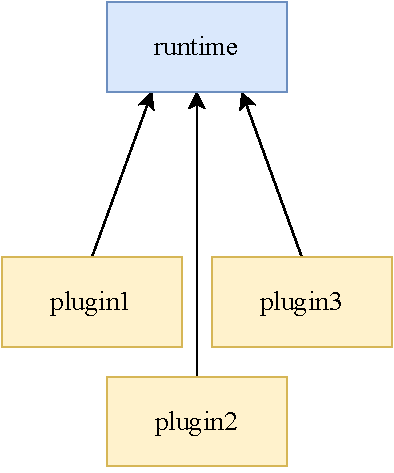
\includegraphics[width=6cm]{./Imagenes/separation-temporary.pdf}
    \caption{Ejemplo de uso de Tremor}%
    \label{fig:separation_temporary}
\end{figure}

\begin{figure}
    \centering
    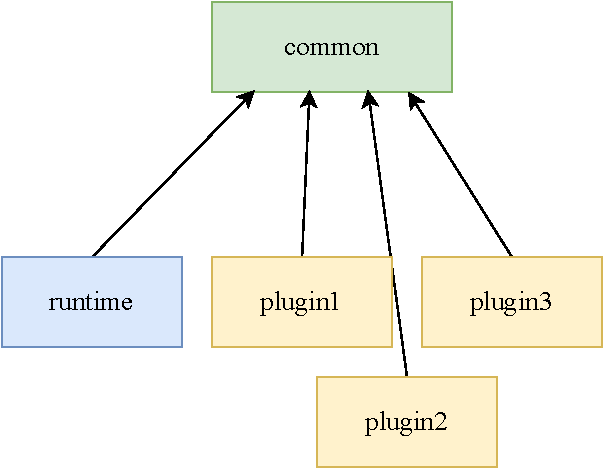
\includegraphics[width=7cm]{./Imagenes/separation.pdf}
    \caption{Ejemplo de uso de Tremor}%
    \label{fig:separation}
\end{figure}

\begin{figure}
    \centering
    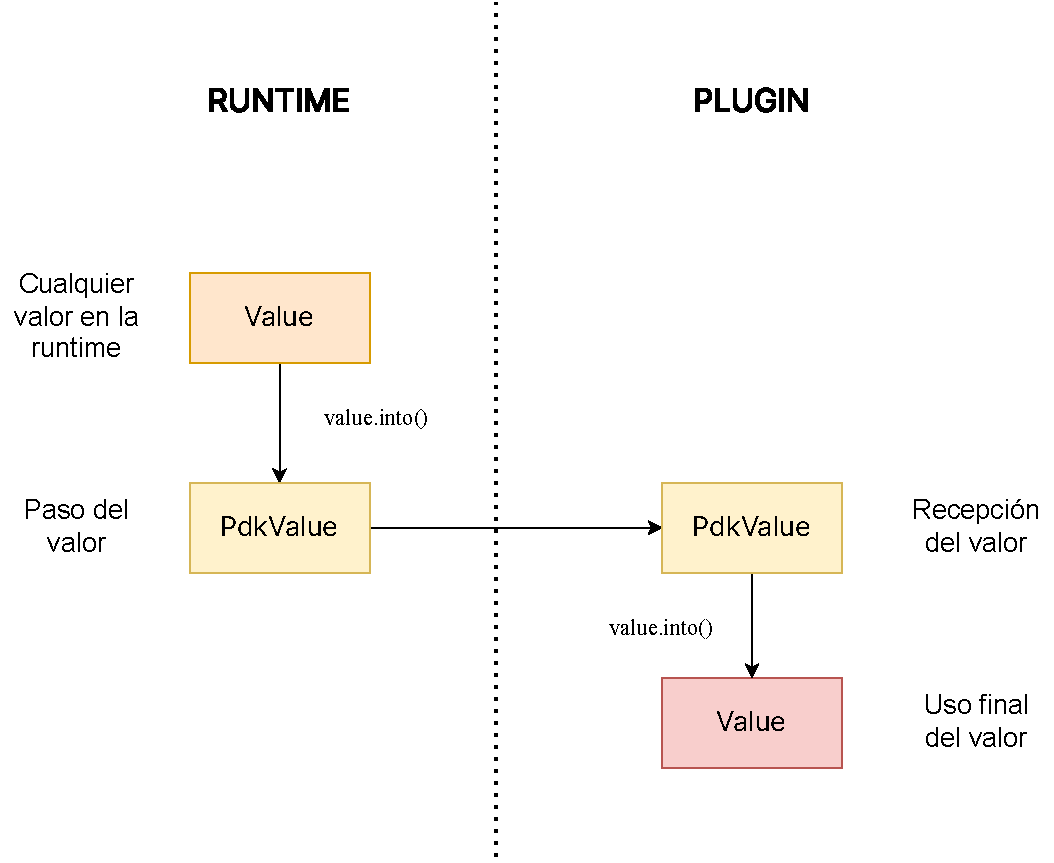
\includegraphics[width=\textwidth]{./Imagenes/simplify.pdf}
    \caption{Ejemplo de uso de Tremor}%
    \label{fig:simplify}
\end{figure}
